%/*% pdflatex -file-line-error -interaction nonstopmode %

\documentclass{article}
\usepackage{graphicx}
\graphicspath{ {./images/} }
\usepackage{amsmath}
\usepackage{amsfonts}
\usepackage{bookmark}
\usepackage{exercises}
\usepackage{amsthm}
\usepackage{yhmath}
\newcommand*{\oldneg}{\mathord{\sim}}

\theoremstyle{definition}
\newtheorem{definition}{Definition}

\setlength{\parindent}{.5in}
\setlength{\parskip}{12pt}

\title{1.6 Exercises}
\begin{document}
\maketitle

\section*{1}
The complex conjugate of $a-bi$ is $a+bi$.

\section*{2}
A complex number is defined to be of the form $a+bi$ where $a$ and $b$ are real numbers. The imaginary unit $i$ is defined to 
be $\sqrt{-1}$. Well, if $b=0$, then by the zero product property, $bi=0$, and thus, the complex number $a+bi$ would simplify to $a$, 
which was assumed to be a real number. Thus, the answer to the question is no.

\section*{3}
$x^2=-28\newline\rightarrow x=\sqrt{-28}=\pm 2i\sqrt{7}$

\section*{4}
$r^2=-624\newline\rightarrow r=\sqrt{-624}=\pm 4i\sqrt{39}$

\section*{5}
$z^2+8=4\newline\rightarrow z=\sqrt{-4}=\pm 2i$

\section*{6}
$s^2-22=-112\newline\rightarrow s=\sqrt{-90}=\pm 3i\sqrt{10}$

\section*{7}
$2x^2+31=9\newline\rightarrow x=\sqrt{-11}=\pm i\sqrt{11}$

\section*{8}
$9-4y^2=57\newline\rightarrow y=\sqrt{-12}=\pm 2i\sqrt{3}$

\section*{9}
$6t^2+5=2t^2+1\newline\rightarrow t=\sqrt{-1}=\pm i$

\section*{10}
$3p^2+7=-9p^2+4\newline\rightarrow 12p^2=-3\newline\rightarrow p=\sqrt{-15}=\pm i\sqrt{15}$

\section*{11}
$-5(n-3)^2=10\newline\rightarrow (n-3)^2=-2\newline\rightarrow n=3\pm i\sqrt{2}$ 

\section*{12}
$(6-3i)+(5+4i)\newline\rightarrow =11+i$

\section*{13}
$(9+8i)+(8-9i)\newline\rightarrow =17-i$

\section*{14}
$(-2-6i)-(4-6i)\newline\rightarrow =-6$

\section*{15}
$(-1+i)-(7-5i)\newline\rightarrow =-8+6i$

\section*{16}
$(8+20i)-(-8+12i)\newline\rightarrow =16+8i$

\section*{17}
$(8-5i)-(-11+4i)\newline\rightarrow =19-9i$

\section*{18}
$(10-2i)+(-11-7i)\newline\rightarrow =-1-9i$

\section*{19}
$(14+3i)+(7+6i)\newline\rightarrow =21+9i$

\section*{20}
$(-1+4i)+(-9-2i)\newline\rightarrow -10+2i$

\section*{21}
C

\section*{22}
$6i(3+2i)=18i+12i^2=18i-12=-12+18i$

\section*{23}
$-i(4-8i)=-4i+8i^2=-8-4i$

\section*{24}
$(1-i)^3=(1-i)(1-i)(1-i)=-2i(1-i)=-2i+2i^2=-2-2i$

\section*{25}
$(-2+5i)(-1+4i)=-18-13i$

\section*{26}
$(-2i)^4=16i^4=16$

\section*{27}
$(8-3i)(8+3i)=73$

\section*{28}
$\frac{7i}{8+i}=\frac{(7i)(8-i)}{(8+i)(8-i)}\newline\rightarrow =\frac{7+56i}{65}\newline\rightarrow =\frac{7}{65}+\frac{56}{65}i$

\section*{29}
$\frac{6i}{3-i}=\frac{6i(3+i)}{(3-i)(3+i)}\newline\rightarrow =\frac{-6+18i}{10}\newline\rightarrow =-\frac{3}{5}+\frac{9}{5}i$

\section*{30}
$\frac{-2-5i}{3i}=\frac{(-2-5i)-3i}{3i(-3i)}\newline\rightarrow =\frac{-15+6i}{9}\newline\rightarrow =-\frac{5}{3}+\frac{2}{3}i$

\section*{31}
$\frac{4+9i}{12i}=\frac{(4+9i)(-12i)}{12i(-12i)}\newline\rightarrow =\frac{108-48i}{-144}\newline\rightarrow =-\frac{3}{4}+{1}{3}i$

\section*{32}
$\frac{7+4i}{2-3i}=\frac{(7+4i)(2+3i)}{(2-3i)(2+3i)}\newline\rightarrow =\frac{2+29i}{13}\newline\rightarrow =\frac{2}{13}+\frac{29}{13}i$

\section*{33}
$\frac{-1-6i}{5+9i}=\frac{(-1-6i)(5-9i)}{(5+9i)(5-9i)}\newline\rightarrow =\frac{-59-21i}{106}\newline\rightarrow =-\frac{59}{106}-
\frac{21}{106}
i$

\section*{34}
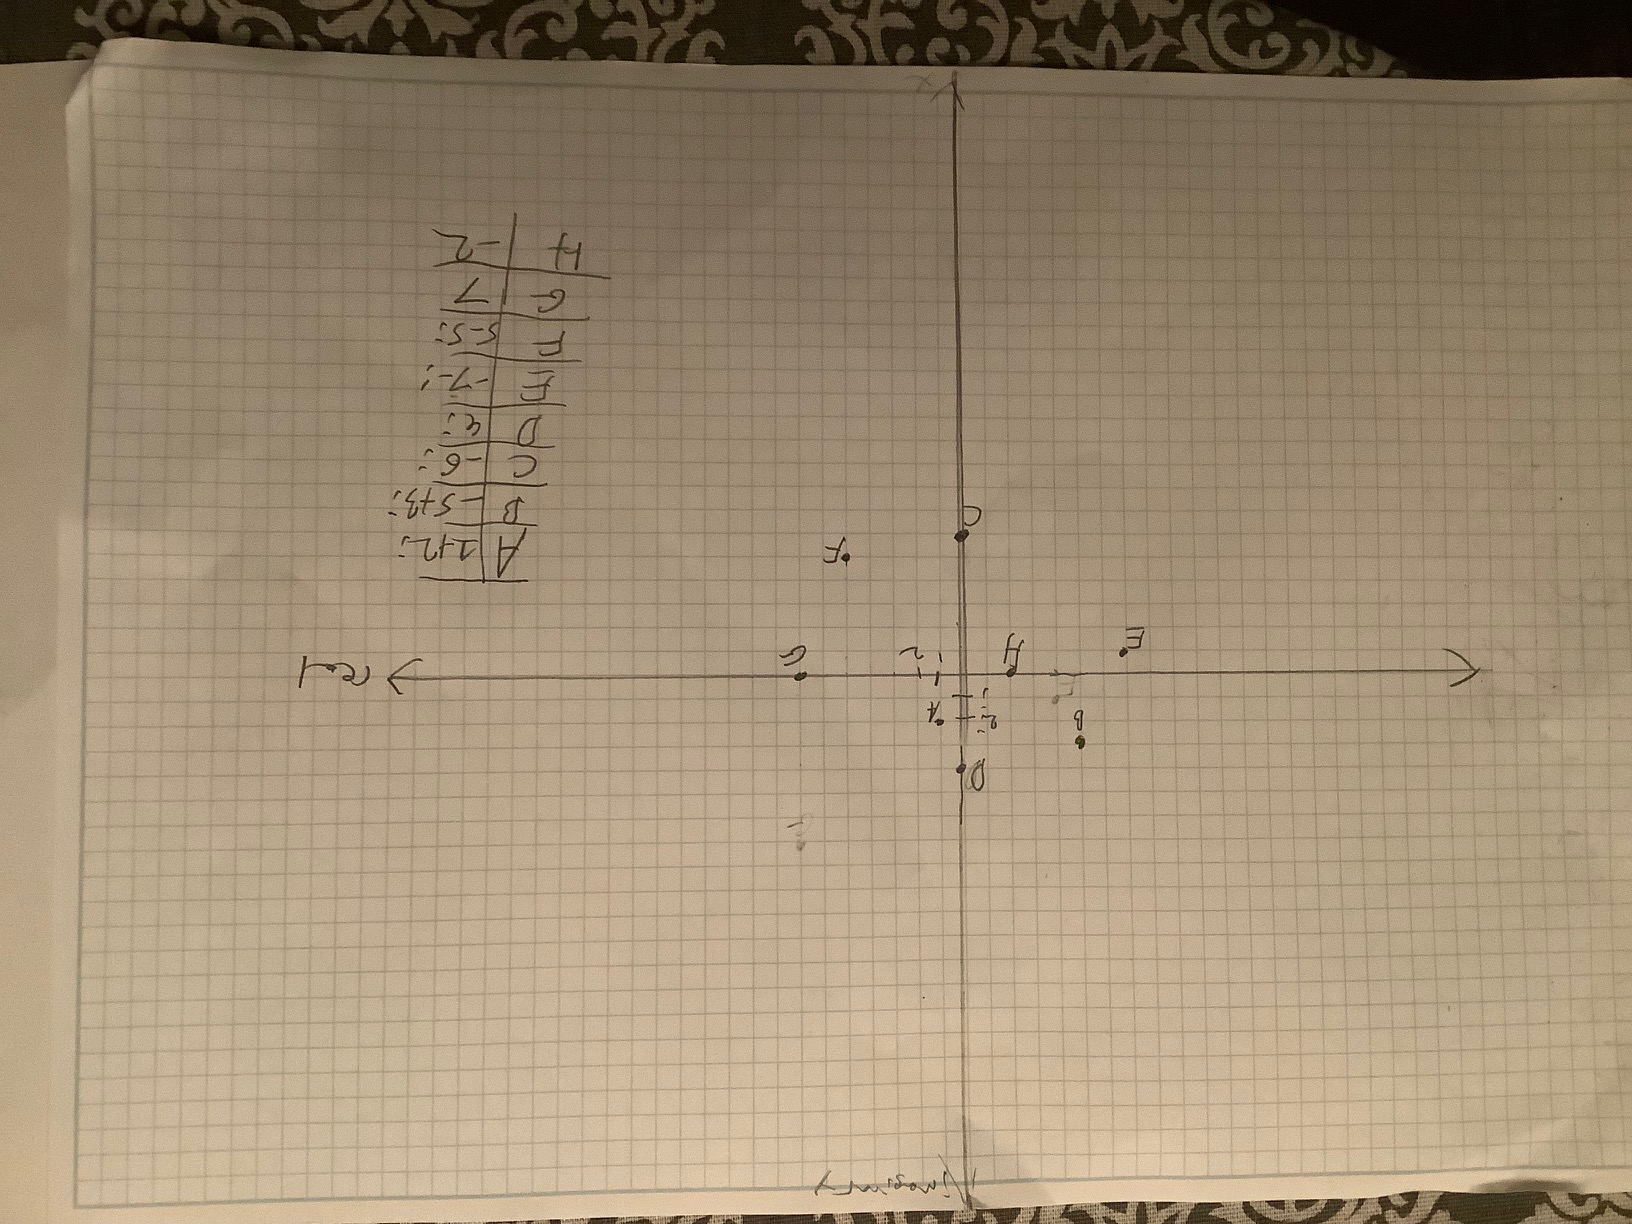
\includegraphics[width = 4in, height = 4in, angle = 180]{picture5}

\section*{42}
$4+3i\newline\rightarrow \sqrt{4^2+3^2}=5$

\section*{43}
$-3+10i\newline\rightarrow \sqrt{(-3)^2+10^2}=\sqrt{109}$

\section*{44}
$10-7i\newline\rightarrow \sqrt{10^2+(-7)^2}=\sqrt{149}$

\section*{45}
$-1-6i\newline\rightarrow \sqrt{(-1)^2+(-6)^2}=\sqrt{37}$

\section*{46}
$-8i=0-8i\newline\rightarrow \sqrt{0^2+(-8)^2}=\sqrt{64}=8$

\section*{47}
$4i=0+4i\newline\rightarrow \sqrt{0^2+4^2}=\sqrt{16}=4$

\section*{48}
$-4+i\newline\rightarrow \sqrt{(-4)^2+1^2}=\sqrt{17}$

\section*{49}
$7+7i\newline\rightarrow \sqrt{7^2+7^2}=\sqrt{98}=7\sqrt{2}$

\section*{50}
$9+12i\newline\rightarrow \sqrt{9^2+12^2}=\sqrt{225}=15$, so the answer is $B$.

\section*{51}
$-8-(3+2i)-(9-4i)\newline\rightarrow =-20+i$

\section*{52}
$(3+2i)+(5-i)+6i\newline\rightarrow =8+7i$

\section*{53}
$5i(3+2i)(8+3i)\newline\rightarrow =(-10+15i)(8+3i)=-125+90i$

\section*{54}
$(1-9i)(1-4i)(4-3i)\newline\rightarrow =(-35-13i)(4-3i)=-179+53i$

\section*{55}
$\frac{(5-2i)+(5+3i)}{(1+i)-(2-4i)}=\frac{10+i}{-1+5i}\newline\rightarrow =\frac{(10+i)(-1-5i)}{(-1+5i)(-1-5i)}\newline\rightarrow 
=\frac{-5-51i}{26}=-\frac{5}{26}-\frac{51}{26}i$

\section*{56}
$\frac{(10+4i)-(3-2i)}{(6-7i)(1-2i)}=\frac{7+6i}{-8-19i}\newline\rightarrow =\frac{(7+6i)(-8+19i)}{(-8-19i)(-8+19i)}\newline\rightarrow 
=\frac{-170+66i}{425}=-\frac{170}{425}+\frac{66}{425}i$

\section*{57}
This answer is not in standard form. $-2i^2=2$, and thus the answer can be corrected to $6+7i$.

\section*{58}
This answer forgets to put parenthesis around $-3$ when it is being squared. Corrected, the answer is:\newline
$\sqrt{2^2+(-3)^2}=\sqrt{13}$

\section*{59}
(a): Additive inverse: $-2-i$ Multiplicative inverse: $z=\frac{1}{2+i}\newline\rightarrow =\frac{1(2-i)}{(2+i)(2-i)}\newline\rightarrow =
\frac{2-i}{5}=\frac{2}{5}-\frac{1}{5}i$\newline
(b): Additive inverse: $-5+i$ Multiplicative inverse: $z=\frac{1}{5-i}\newline\rightarrow =\frac{1(5+i)}{(5-i)(5+i)}\newline\rightarrow =
\frac{5+i}{26}=\frac{5}{26}+\frac{1}{26}i$\newline
(c): Additive inverse: $1-3i$ Multiplicative inverse: $z=\frac{1}{-1+3i}\newline\rightarrow =\frac{1(-1-3i)}{(-1+3i)(-1-3i)}\newline
\rightarrow =\frac{-1-3i}{10}=-\frac{1}{10}-\frac{3}{10}i$

\section*{60}
$2+6i$ and $-4-6i$ are two such examples. These numbers are related such that, if we let $b_1=6$ and $b_2=-6$ in the above two 
imaginary numbers, $b_1+b_2=0$.

\section*{61} 
$\frac{a+bi}{c+di}\newline\rightarrow =\frac{(a+bi)(c-di)}{(c+di)(c-di)}\newline\rightarrow =\frac{(ac+bd)+(bc-ad)i}{c^2+d^2}
\newline\rightarrow
 =
\frac{ac+bd}{c^2+d^2}+\frac{bc-ad}{c^2+d^2}i$

\section*{62}
$\frac{a-bi}{c-di}\newline\rightarrow =\frac{(a-bi)(c+di)}{(c-di)(c+di)}\newline\rightarrow =\frac{(ac+bd)+(ad-bc)i}{c^2+d^2}\newline
\rightarrow =
\frac{ac+bd}{c^2+d^2}+\frac{ad-bc}{c^2+d^2}i$

\section*{63}
$\frac{a+bi}{c-di}\newline\rightarrow =\frac{(a+bi)(c+di)}{(c-di)(c+di)}\newline\rightarrow =\frac{(ac-bd)+(ad+bc)i}{c^2+d^2}\newline
\rightarrow =
\frac{ac-bd}{c^2+d^2}+\frac{ad+bc}{c^2+d^2}i$

\section*{64}
$\frac{a-bi}{c+di}\newline\rightarrow =\frac{(a-bi)(c-di)}{(c+di)(c-di)}\newline\rightarrow =\frac{(ac-bd)+(-ad-bc)i}{c^2+d^2}\newline
\rightarrow =\frac{ac-bd}{c^2+d^2}+\frac{-ad-bc}{c^2+d^2}i$

\section*{65}
$Impendance =4+6i-9i=4-3i$

\section*{66}
$Impendance =14+7i-8i=14-i$

\section*{67}
$Impendance =12+8i-10i-6i=12-8i$

\section*{68}
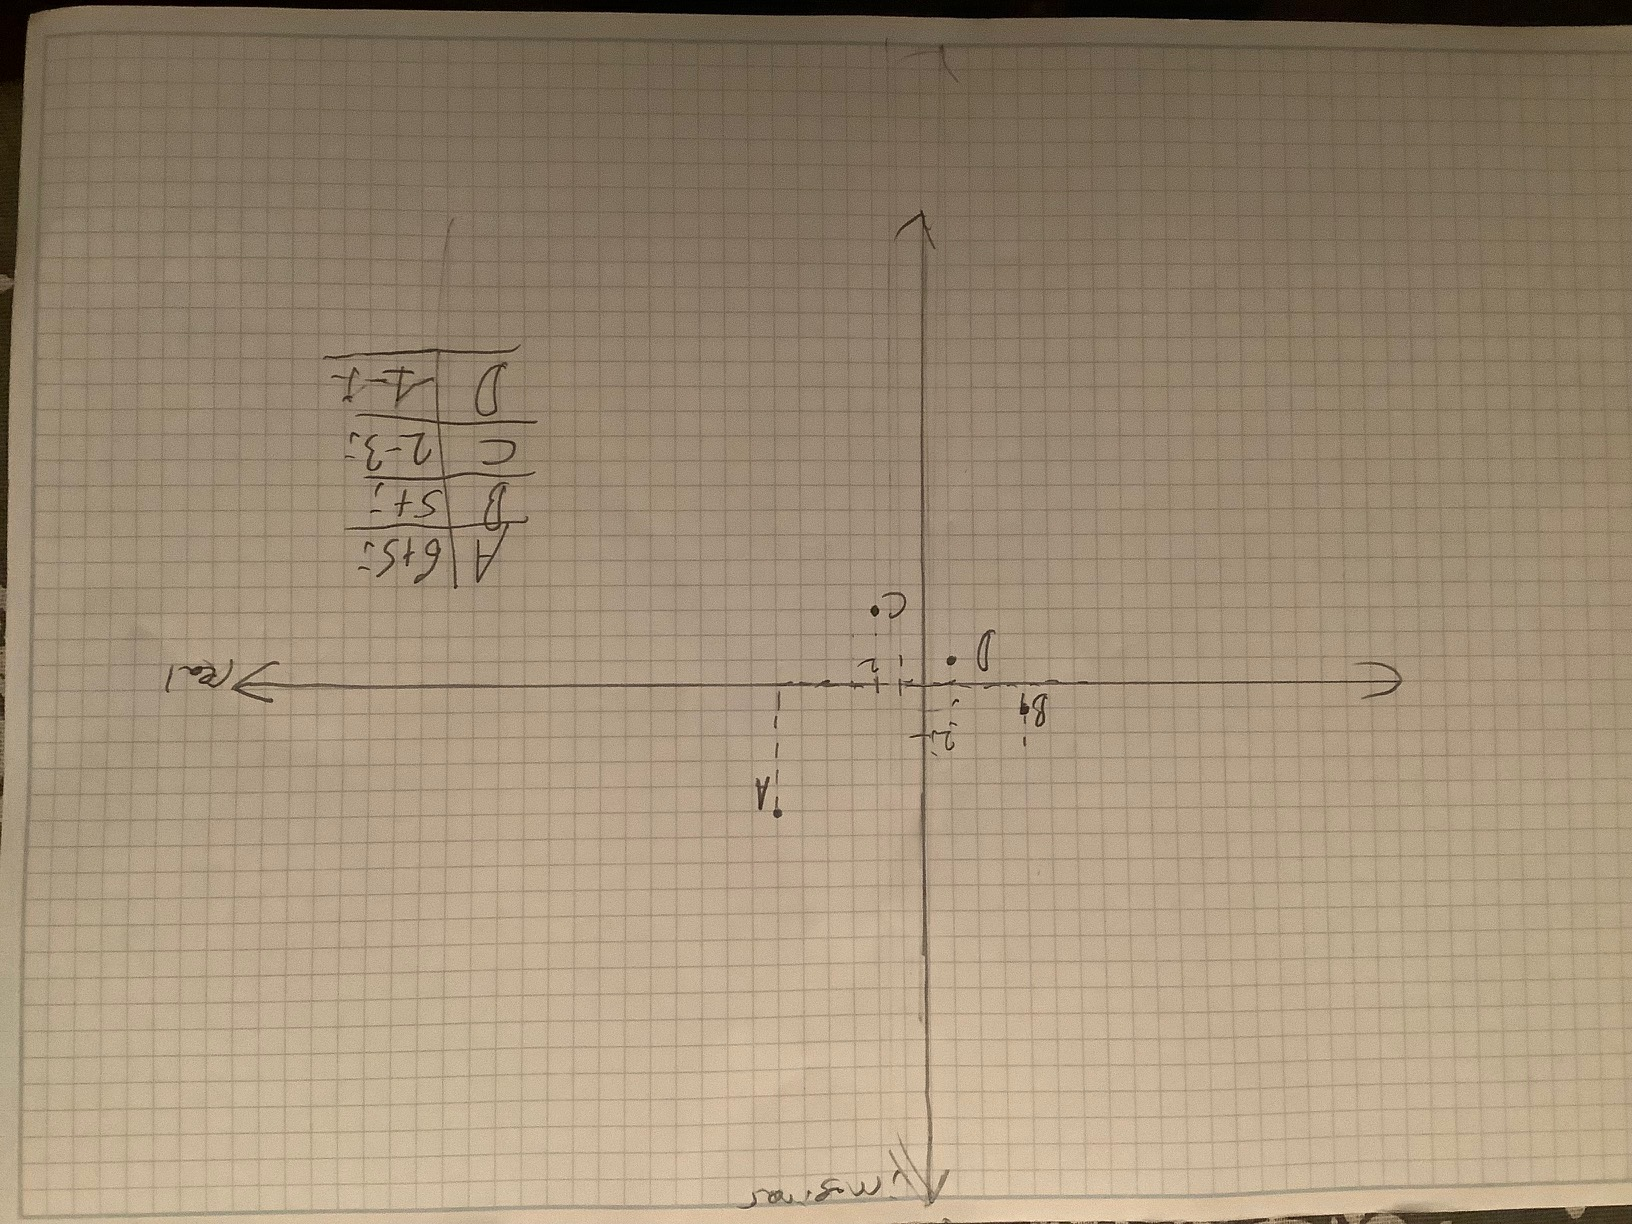
\includegraphics[width = 4in, height = 4in, angle = 180]{picture4}

\section*{69}
\begin{table}[h!]
        \begin{center}
                \begin{tabular}{l|c|c|c|c|c|c|r}
                        $i^1$ & $i^2$ & $i^3$ & $i^4$ & $i^5$ & $i^6$ & $i^7$ & $i^8$\\
                        \hline
                        $i$ & $-1$ & $-i$ & $1$ & $i$ & $-1$ & $-i$ & $1$
                \end{tabular}
        \end{center}
\end{table}
The pattern that can be concluded from this table is that the series of infinite powers of $i$ alternates from $i$ to $-1$ to $-i$ 
to $1$ to $i$, and then the pattern restarts. The next four powers of $i$ are $i,\ -1,\ -i,\ 1$.

\section*{70}
The communtative property of multiplication states that $a\times b=b\times a$.\newline
$(4-2i)(-3+i)=-12+4i+6i-2i^2=-10+10i$\newline $(-3+i)(4-2i)=-12+6i+4i-2i^2=-10+10i$

\section*{71}
The associative property of multiplication states that $(a\times b)\times c=a\times (b\times c)$.\newline
$((7-2i)i)(-1+i)=(2+7i)(-1+i)=-2+2i-7i+7i^2=-9-5i$\newline $(7-2i)(i(-1+i))=(7-2i)(-1-i)=-7-7i+2i+2i^2=-9-5i$

\section*{72}
The distributive property states that $a(b+c)=ab+ac$.\newline
$-2i((3+2i)+(5+i))=-2i(8+3i)=6-16i$\newline $-2i(3+2i)-2i(5+i)=(4-6i)+(2-10i)=6-16i$

\section*{73}
The commutative property of addition states that $a+b=b+a$.\newline
$(a+bi)+(c+di)=a+c+(b+d)i$\newline $(c+di)+(a+bi)=a+c+(b+d)i$

\section*{74}
$\sqrt{-4}\times \sqrt{-25}=2i\times 5i=-10$ while $\sqrt{100} = 10$. This suggests the fact that $\sqrt{a}\times \sqrt{b}\ne \sqrt{ab}$ 
when $a$ and $b$ are negative numbers.

\section*{75}
(a): $Z=\frac{(4+5i)(7-3i)}{(4+5i)+(7-3i)}=\frac{43+23i}{11+2i}=\frac{(43+23i)(11-2i)}{(11+2i)(11-2i)}\newline\rightarrow =
\frac{519+167i}{125}=\frac{519}{125}+\frac{167}{125}i$\newline
(b): $Z=\frac{(6+8i)(10-11i)}{(6+8i)+(10-11i)}=\frac{148+14i}{16-3i}=\frac{(148+14i)(16+3i)}{(16-3i)(16+3i)}\newline\rightarrow =\frac 
{2326+668i}{265}=\frac{2326}{265}+\frac{668}{265}i$\newline
(c: $Z=\frac{(3+i)(4-6i)}{(3+i)+(4-6i)}=\frac{18-14i}{7-5i}=\frac{(18-14i)(7+5i)}{(7-5i)(7+5i)}\newline\rightarrow =\frac
{196-8}{74}=\frac{98}{37}-\frac{2}{37}i$

\section*{76}
(a): $f(z_0)=i^2+1+i=i$. Thus, because for every $z_i$, $f(z_i)=i$, the numbers stay in a finite bound, and hence, $z_0$ is a member of 
the Julia set corresponding to $z^2+1+i$.\newline
(b) (I was not sure how to verify for the next 3 that, for all the infinitely many $z_i$, whether $f(z_i)$ stayed in a finite bound, or 
whether these 
did not)
: $f(z_0)=1^1+1+i=2+i$.\newline
(c): $f(z_0)=(2i)^2+1+i=2+i$.\newline
(d): $f(z_0)=(2+3i)^2+1+i=-4+13i$.
\end{document}
